%\documentstyle [11pt]{report} 
\documentclass[10pt]{article} 
\def\inputGnumericTable{}

\usepackage[latin1]{inputenc}
\usepackage[usenames]{color}
\usepackage{array}
\usepackage{longtable}
\usepackage{calc}
\usepackage{multirow}                                         
\usepackage{hhline}                                          
\usepackage{ifthen}

\usepackage{a4}
\usepackage{amssymb}
\usepackage[english]{babel}
\usepackage[normal]{caption2}  
\usepackage{rotating}
\usepackage{graphicx}
\usepackage{dcolumn}
\usepackage{placeins} % per la floatbarrier
%\usepackage[colorlinks=true,bookmarksnumbered=true,citecolor=red,linkcolor=blue,pdfauthor={Laura Sartori},pdftitle={The ApeNEXT project}]{hyperref}
% mettere bookmarksnumbered=false 
% \usepackage{afterpage}

%\usepackage{fancybox}
\usepackage{amssymb} % per il minore
\usepackage{amsmath}
\usepackage{comment}
\usepackage{layout}
%\usepackage{hyperref}
\numberwithin{figure}{section}
\numberwithin{equation}{section}
\numberwithin{table}{section}
\newcommand{\fix}{\textbf{[FIX]}}
\newcommand{\help}{\textbf{[HELP]}}
\newcommand{\Dbar}{\not \!\! D}
\newcommand{\de}{\partial}
\newcommand{\As}{$\mathcal{D}$}
\newcommand{\A}{\As\ }
\newcommand{\Ks}{$\mathcal{K}$}
\newcommand{\K}{\Ks\ }
\newcommand{\0}{\phantom{0}}
\renewcommand{\ni}{\noindent}
\newcommand{\myurl}[1]{\texttt{#1}}
\definecolor{mygreen}{cmyk}{0.64,0,0.95,0.40}
\newcommand{\aqed}{\alpha_\mathit{em}}
\newcommand{\aqcd}{\alpha_\mathit{s}}
\newcommand{\blue}{\color{blue}}
\newcommand{\green}{\color{mygreen}}
\newcommand{\red}{\color{red}}
\newcommand{\black}{\color{black}}
\newcommand{\vstr}{\vspace{\stretch{1}}}
\newcommand{\mydate}{\def\filedate{10 dicembre 2001}}
\newcommand{\mynodate}{\def\filedate{}}
\newcommand{\coloroval}[2]{{\color{#1}\ovalbox{\color{black}#2}}}

\begin{document} 
\thispagestyle{empty}
\hfill {FTK note number ??}  

\hfill Last Modification: \today  

\hfill Version 1.1 (June 9th, 2012)
\vspace{2cm}
{\center

{\bf \LARGE Fast Track data formats, numbering schemes and internal memories}
\vspace{1cm}
%\arabic{footnote}

%%\addtocounter{footnote}{1}
%%\footnotetext{University of Pisa - Physics departement}
\large 
%\author {
%%A. Annovi\footnotemark[1] \footnotemark[2] \\
\vspace{1cm}
%\date  {}
%DRAFT -
 }
\vspace{2cm}

%==================================================================
\begin{abstract}
%This note describes the technical details of the AMchip03 implementation.
This note is the data format for internal Fast Track communication for Fast Track I/O from RODs and to ROSes.
\end{abstract}

%\include{prima}
%\maketitle  
\bibliographystyle{plain}
\baselineskip 16pt % line spacing-24pt for double spacing
%\hoffset 15mm
%\voffset -4mm
%\newpage
%\mbox{}
\newpage

\tableofcontents
\newpage

\section{Change log} 

\begin{enumerate}
\item[1.1] Changed FTK\_IM to EDRO format to avoid problems with LSBs
\end{enumerate}

\section{Introduction} 
Here we define a general data format for the Fast Tracker (FTK) project and the details of all internal data formats.
Each communication channel in FTK being either a board-to-board communication or a chip-to-chip communication should be documented here.

All data transfer in FTK should follow a common standard. It has to be simple and flexible for the different uses in FTK.
We have 3 different hardware layer for communications:
\begin{itemize}
\item electrical parallel bus
\item S-Link 
\item SNAP12
\end{itemize}

For communication over electrical parallel buses we use a protocol ispired to the SVT data format shown in table~\ref{tab:generic_format}.
This is generic data format for FTK data transfers.
Data is organized into events and within events into packets. The last word of each packet is identified by ``End Packet'' bit (EP) equal to 1.
Each event starts with an header packet identified as the first packet of the event.
It is followed by a variable number of packets and then by an end event packet identified by ``End Event'' bit (EE) equal to 1 for all words of the packet.

\begin{table}[h]
\begin{tabular}{c|c|c|l}
control signals & EE & EP & data word    \\ \hline \hline
CLK, DV, HOLD and FREEZE & 0 & 0 & header data word 1 \\
 "   " & 0 & 1 & header data word 2 \\ \hline
 "   " & 0 & 0 & data packet 1 word 1 \\ 
 "   " & 0 & 1 & data packet 1 word 2 \\  \hline
 "   " & 0 & 1 & data packet 2 word 1 \\ \hline
 "   " & 0 & 1 & data packet 3 word 1 \\ \hline
 "   " & 0 & 0 & data packet 4 word 1 \\ 
 "   " & 0 & 0 & data packet 4 word 2 \\ 
 "   " & 0 & 1 & data packet 4 word 3 \\ \hline
 "   " & 1 & 0 & end event data word 1 \\
 "   " & 1 & 1 & end event data word 2
\label{tab:generic_format}
%%\caption{  Generic data format for all FTK data trasfers}
\end{tabular}
\end{table}

Several things are not specified at this time (October 2010) and may differ among the different communication channels in FTK.
Packets don't have a fixed number of data words. The actual packet length is to be specified for each communication channel.
The size of the data word is not specified either. It will be tailored for each communication.
However we set a minimum of 16 bits for all communication channels.
This allows for packing standard 32bits word in no more that 2 data words.

All data transfer are synchronous on the rising clock edge with ``Data Valid'' (DV) and ``HOLD'' control signals.
When data transfers use optical links or electrical serializer/deserializer protocols, it is intended that interface with the optical links or serializer/deserializer will use be synchronous on the rising clock edge with ``Data Valid'' (DV). The ``HOLD'' and ``FREEZE'' signals travel in the opposite direction. They might need special care.
For example input S-Links to FTK, which run from the RODs to the Data Formatter boards, use a dedicated fiber for XON/XOFF.
The transmitter board will respond to a ``HOLD'' signal stopping data trasfers within a few clock cycles. 
For this reason the receiving board should assert ``HOLD'' well before the FIFOs are full, for example genereting ``HOLD'' from ``FIFO\_almost\_full'' signal.
When the receiving board issues the ``FREEZE'' signal the transmitting board should freeze the corresponding spybuffers.

\subsubsection{SLink}

Other communication will use the SLink protocol.
Data in the SLink protocol will represent the data packets.
The begin and end of an event will be marked by SLink control words.


\subsection{End Event packet}
This section is under construction. For the moment we keep a (partial) list of information that should appear in the EE packet. When the list will be complete we shold define the EE packet in detail.

\begin{itemize}
\item forward\_FREEZE: tells the down-stream boards to freeze this event
\item error bits: to be defined
\end{itemize}

\section{Specific Data Formats}
\subsection{Pixel and SCT RODs output formats}

\begin{figure}
\begin{center}
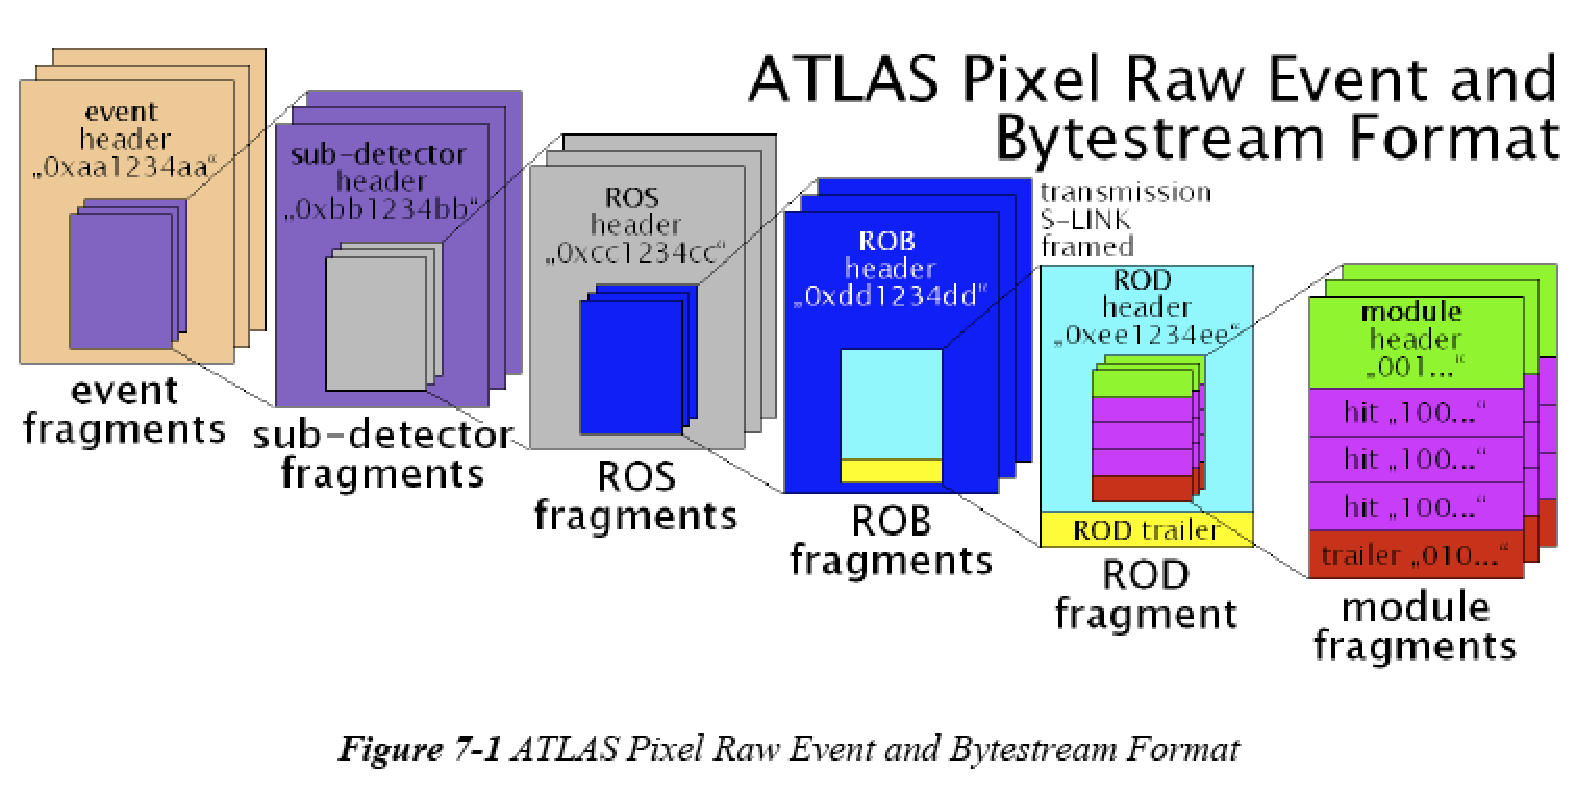
\includegraphics[width=\textwidth]{figs/PIXEL_ROD_format_2.pdf}
\end{center}
\caption{\label{fig:pixel_bytestream}Pixel bytestream in the ATLAS bytestream.}
\end{figure}

\begin{figure}
\begin{center}
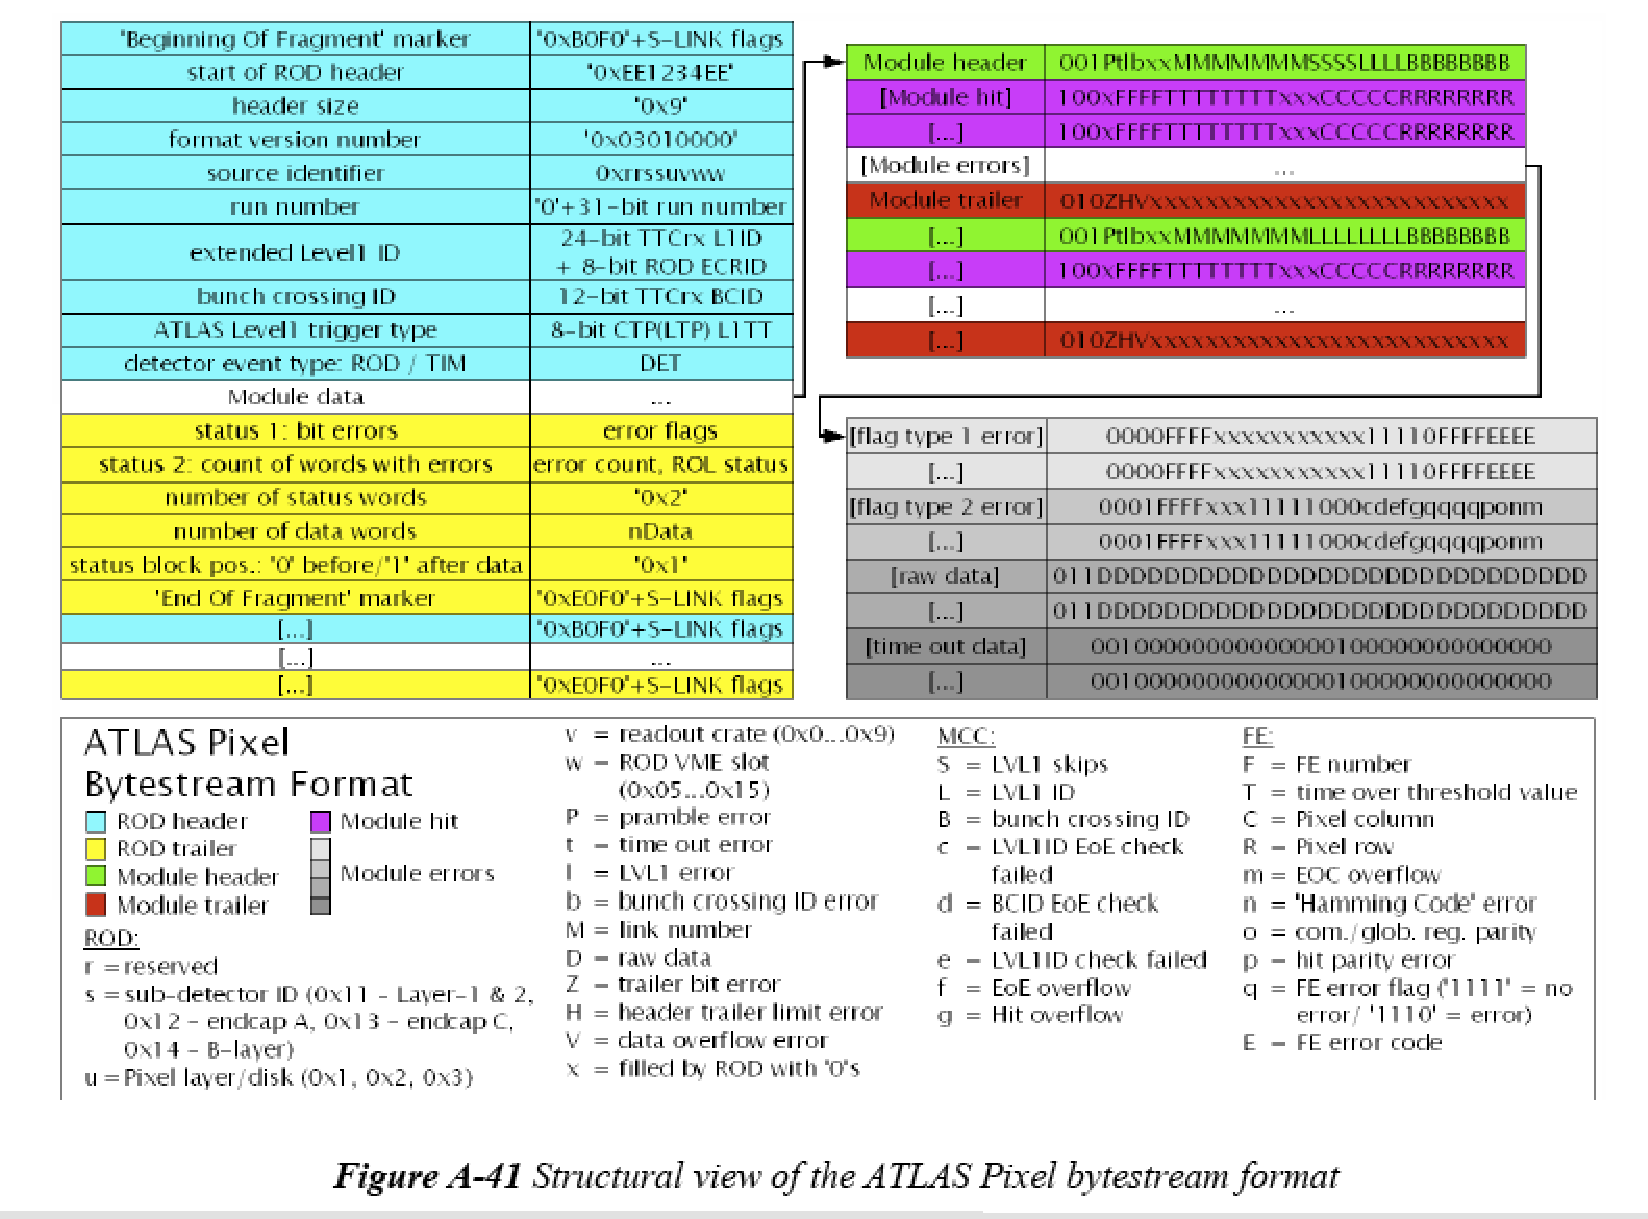
\includegraphics[width=\textwidth]{figs/PIXEL_ROD_format_1.pdf}
\end{center}
\caption{\label{fig:pixel_detailed_format}Pixel data format.}
\end{figure}

Figures~\ref{fig:pixel_bytestream} and~\ref{fig:pixel_detailed_format} are taken from http://cds.cern.ch/record/1092108/files/CERN-THESIS-2008-022.pdf.



SCT ROD data format is shown in talbe~\ref{fig:sct_rod_format} from ROD User Manual [http://www-eng.lbl.gov/~jmjoseph/Atlas-SiROD/Manuals/usersManual-v164.pdf].
\begin{figure}
\begin{center}
\includegraphics[width=\textwidth]{figs/SCT_ROD_format.pdf}
\end{center}
\caption{\label{fig:sct_rod_format}SCT data format.}
\end{figure}







\clearpage
\subsection{Clustering mezzanine output for DataFormatter}
\label{FTK_IM_Output}
Both Pixel and SCT channels will output data in this format:

\begin{table}[h]
\begin{tabular}{c|c|c|c|c|c|c|c|c|l}
32 & 31..28 & 27..24 & 23..20 & 19..16 & 15..12 & 11..8 & 7..4 & 3..0 & comment\\ \hline
  1 & B & 0 & F & 0 & x & x & x & x & begin of fragment\\\hline
  0 & C & A & F & E & \multicolumn{4}{c|}{reserved (15..0)} & header word 1\\\hline
  0 & \multicolumn{8}{c|}{LVL1ID (31..0)} & header word 2 \\ \hline
  0 & \multicolumn{8}{c|}{0 + 31-bit run number (30..0)} & header word 3 \\ \hline
  0 & 0 & 0 & \multicolumn{2}{c|}{L1TT (23..16)} & 0 &  \multicolumn{3}{c|}{TTCrcBCID (11..0)}  & header word 4\\ \hline
  0 & \multicolumn{8}{c|}{reserved (31..0)}  & header word 5 \\ \hline
  0 & \multicolumn{8}{c|}{\textbf{DATA} (31..0)}  & data words \\ \hline
  1 & E & 0 & D & A & x & x & x & x & end of data\\\hline
  0 & \multicolumn{8}{c|}{LVL1ID (31..0)} & trailer word 1\\ \hline
  0 & \multicolumn{8}{c|}{error flags (31..0)} & trailer word 2\\\hline 
  0 & \multicolumn{8}{c|}{reserved (31..0)} & trailer word 3\\ \hline
  0 & \multicolumn{8}{c|}{CRC (31..0)} & checksum \\ \hline
  1 & E & 0 & F & 0 & x & x & x & x & end of fragment \\\hline
\end{tabular}
\caption{\label{tab:clustering_output}Clustering mezzanine output for each of the 4 input/output channels toward the Data Formatter. Bit 32 is the control word flag. The CRC will be calcuated over all header, data and trailer words in the event. It will exclude control words and the CRC itself.}
\end{table}

\begin{table}[h]
\begin{tabular}{c|c|c|c|c|c|c|c|c|c|l}
  31 & 30..28 & 27 & 26..16 & 15 & 14 & 13 & 12 & 11 & 10..0 & comment\\ \hline
  1 & rrr & \multicolumn{2}{c|}{reserved} & 0 & \multicolumn{3}{c|}{rrr} & r & module num. & Pixel module\\\hline

  0 & c.width & \multicolumn{2}{c|}{column coord} &
  r & r & \multicolumn{2}{c|}{r.width} & \multicolumn{2}{c|}{row coord} & Pixel cluster1\\\hline
  1 & rrr & \multicolumn{2}{c|}{reserved} & 
  1 & r & r &\multicolumn{3}{c|}{module num.} & SCT module\\\hline

  0 & H2 width &
  H2 empty & Hit2 coord &
  r & \multicolumn{3}{c|}{H1 width} & r & Hit1 coord & SCT cluster1\\\hline

\end{tabular}
\caption{\label{tab:FTK_IMdataWords} Data format for clustering mezzanine data words. All numbers are bits. The 'r' is a reserved bit.}
\end{table}

\newpage
\section{FTK numbering schemes}

This section is in progress. It should contain the definition of all numbering internal to FTK.
FTK should use a global ID for each detector module (most likely already defined by offline).
Within each $\eta-\phi$ tower we should define a local ID in order to reduce the memory usage.

For the vertical slice the region map defined by tower is stored in file ``TrigFTKSim/config/map\_file/vertical\_slices.rmap''. Description for the fields in this file is available in file ``TrigFTKSim/config/map\_file/vertical\_slices.rmap.COMMENT''.

The format is: 
\begin{verbatim}
#PIX ENDCAP PHYSICAL_LAYER MIN_PHI MAX_PHI N_PHI MIN_ETA MAX_ETA N_ETA 
0
1       0       0       -1      -1      22      -1      -1      13
1       0       1       8       11      38      0       6       13
\end{verbatim}

For each logical layer we must calculate a "local module ID" that is used to calculate the SS within a tower.
\[ SStower = "local module ID" * maxSSmodule + SSmodule \]
Where maxSSmodule is the maximum number of superstrips within a module,
SSmodule is the local superstrip number calculated within a module.

For the vertical slice the "local module ID"  is calculated starting from data in the map file in this way: \\
local module ID 0 is the one with the least phi number and least eta number.\\
module ID id calculated as \\
local module ID = localEta*nphi+localPhi; \\
where localEta = eta-MIN\_ETA; \\
localPhi = phi-MIN\_PHI; (accounting for wrap around 2pi) \\
nphi = MAX\_PHI - MIN\_PHI +1; (accounting for wrap around 2pi) 

\newpage

\section{FTK memories}
Here we should describe all memories internal to FTK.

\subsection{FTK\_IM memories}
\subsubsection{FTK\_IM module map}
The FTK\_IM module map will identify modules in data received from the RODs and it will number modules by hashID.
In the input data, modules are identified by the sourceid (word 4 of the ROD header) which uniquely identifies the ROD and by the link number.
For Pixels the link number is written in bits 22:16 of each module header word. See figure~\ref{fig:pixel_detailed_format}.
For SCT the link number is written in bits 7:0 of each 16 bits module header packets packed in 32 bit word.
The hashID is a number that counts pixel modules, and separately strip modules.
It has the advantage that it uses the minimum number of bits to store this information. The hashID will be used throughout FTK to refer to a module after the conversion performed in the FTK\_IM. This hashID is the same as the offline hashID.

For both Pixel and SCT, the FTK\_IM will use a look up table (LUT), also called module\_LUT or modLUT, in order to convert the sourceid and link number into a hashID.
The sourceid will be coded into the LUT during FTK\_IM configuration. Each FTK\_IM channel will have its own moduleLUT configured specifically for the ROD that will be connected to it.
The link number will be used as address to access the modLUT. The output data of the module LUT will be a 16 bit words that corresponds to the least 16 significant bits of the module words in table~\ref{tab:FTK_IMdataWords}, including the pixel/SCT (SCT=1) bit. For SCT, bit 13 will be used for the flag of module that reversed strip number.
Link numbers that are not associated to module will be set to the invalid module number represented by all bits set to 1. This is 0x7FF for Pixels and 0x1FFF for SCT.
The link number is a 7 bit number. The module LUT in the firmware will have an 8 bit address with most significant bit always set to 0. 

\subsubsection{Summary}
\begin{table}[h]
\begin{tabular}{l|ccc}
memory name & depth & x & word size \\ \hline
module LUT & 256 & x & 16 bits \\
\end{tabular}
\caption{\label{tab:FTK_IMmems}Size of the FTK\_IM memories}
\end{table}


\subsection{Data Organizer memories}
In the description below I'm keeping 3 options open.

1) we use the SS offset from 4.1.1 and then the SSmap will not need the local module ID in input.
     Minimize the memory size.

2) we use the local module ID. In this case the SS offset is not needed ONLY if we assume the same SS definition for all modules in a logical layer.
    Largest memory requirements.

3) A compromise (I think a good one given that we have not yet simulated different SS mapping in the same layer)
     is to have a few bits (e.g. 2) for the local module ID.
     Those bits would defined 1 out of 4 possible SS mapping for a module.
     In this case the SS offset is needed.

\subsubsection{Module map}
This memory will map a global module ID to a local module ID, a logical layer and the $SS_{offset}$ for the given module.
This memory will be a small one. The total number of modules in the system is below 8k. This will be the memory depth. \\
The local module ID, corresponding to one memory word, will be defined as: \\
25:20 local module ID \\
19:16 logical layer number for the given module \\
15:0 super-strip offset for the given module.

The ``hitToModuleId'' function in TrigFTKSim/src/atlClusteringLNF.cxx encodes the module ID in a 16 bits word, that requires a 64k location deep memory. Further reduction is possible.

\subsubsection{Global module ID}
The global module ID (or simply moduleID) is defined in a function ...
It is calculated counting starting from 0 the pixel modules, and starting from 4192 the SCT modules.
For both pixel and SCT, the modules are counted starting from the inner barrel layer going to the outer barrel layer.
For each barrel layer, we start counting modules at phi=0 starting from the module at the most negative z (C-side) toward the most positive z (A-side), then the modules with larger phi are counted again going from negative to positive z.
After the barrel, the inner most disk is counted side A first and side C later, then the second inner most disk is counted side A first and side C later, and so on.
For each endcap disk, we start counting modules at phi=0 starting from the module at the inner most module (smallest radius) toward the outer most module (largest radius), then the modules with larger phi are counted again going from inner most module to outer most.

\subsubsection{Super-strip map}
\label{sec:ssmap}
This memory will convert one cluster position into one AM super-strip (SSID). There will be 8 SS maps: one for each logical layer in the AM.
They will be of two kinds, one for pixels and the other for SCT.
The pixels will need a larger memory. The address or input will be the cluster coordinates down to the pixel level using 17 bits (see section~\ref{cluOutput}) plus 6 bits for the local module ID for a depth of $2^{23}=8$M~words. Each word will contain a 16 bits SS.
The SCT will use just 10 bits for the strip number plus 6 bits for the local module ID for a depth of $2^{16}=64$k~words. Each word will contain a 16 bits SS.
The description above allows to use different grouping of pixels and strips into superstrips for each module.
This is desirable to keep flexibility, howerver it may be too demanding.
If required by FPGA constraints, the number of bits allocated for the local module ID can be reduced.
If the local module ID bits in the address of the SS map are reduced from 6 to 2, we would have 4 possibile SS maps (each with 17 bits of addressing covering a full module) for each logical layers.
This should be enough to grant some flexibility. It will allow a reduction of the memory size by a factor of 16 with respect to the use of all 6 bits of local module ID.

\begin{table}[h]
\begin{tabular}{|r|c|c|c|c|c|}
SS kind & 31:26 & 25:20 & 19:16 & 15 & 14:0 \\ \hline
simulation & reserved & 6 care/don't care bits & reserved & reserved & full resultion SSID \\
hardware & N/A & N/A & N/A & reserved & full resolution SSID \\
\end{tabular}
\caption{\label{tab:SSID_bitwise}Definition of SSID in hardware and simulation}
\end{table}

The SCT SSID will be calculated dividing the integer strip number (i.e. discarding the LSB that represent half a strip). The divisor will be used to generate the content of the SS map in software and used to load the SCT SS map during configuration.
The Pixel SS map is slightly more complicated. It will be calculated in this way.
There will be four configuration numbers. Let's call them ($size_{\phi}$, $size_{\eta}$, $group_{\phi}$, $group_{\eta}$).
The initial configuration could be (48, 36, 4, 2).
The local SS number is defined by
\[ max_{\phi} = \frac{328}{size_{\phi}*group_{\phi}} \]
\[ max_{\eta} = \frac{144}{size_{\eta}*group_{\eta}} \]
%%\clearpage
\[ SS_{local} = group_{\phi}*group_{\eta} * \]
\[ ( \, max_{\phi}*\frac{\eta}{size_{\eta}*group_{\eta}} + \frac{\phi}{size_{\phi}*group_{\phi}}\, )  + group_{\phi} * ( \, \frac{\eta}{size_{\eta}} \% \, group_{\eta} \, ) + ( \, \frac{\phi}{size_{\phi}} \% \, group_{\phi} \, ) \]
\[ SS_{global} = SS_{offset} + SS_{local} \]

%%Where the number 8 is a fixed constant that corresponds to 3 bits used in the new 65nm AMchip for the variable resolution.
%%Even if the CDF AMchip doesn't have the variable resolution feature we will start with the final configuration for the SS map.
The thinnest super-strips that have been used in the simulation are (12, 36, 4, 2).
This correspond to $max_{\phi}=7$, $max_{\eta}=2$. So the largest super-strip within a module ($SS_{local}$) would be 7*2*8 = 112.
For example with this configuration, the $SS_{offset}$ would be calculated by the software to be multiples of 112. I.e. $SS_{offset}=112*moduleID_{local}$, where $moduleID_{local}$ is an index for all modules within a logical layer of a single $\eta-\phi$ tower.
Indeed the $SS_{offset}$ must always be a multiple of 8 in order not to mess up the 3 LSBs that are used by the variable resolution logic.
This leaves us room for $2^{15} / 112 \approx 292$ modules for each $\eta-\phi$ tower that are more than enough.
For configurations with large enough super-strip that don't use all SS numbers up to $2^{15}$, we can choose to align $max_{\phi}$ and $max_{\eta}$ to powers of 2 so that all fields end up using well defined bits.
For example the (48, 36, 4, 2) configuration can use:
$ max_{\phi} = 2 $, $max_{\eta} = 2 $ with super-strip offsets multiples of 32. In this case the super-strip word would be: \\
 \\
\begin{tabular}{c|c|c|c|c}
(15:7) & (6:5) & (4:3) & (2) & (1:0) \\ \hline
local module ID & $\frac{\eta}{size_{\eta}*group_{\eta}}$ & $\frac{\phi}{size_{\phi}*group_{\phi}}$ & $\frac{\eta}{size_{\eta}} \% \, group_{\eta}$ & $\frac{\phi}{size_{\phi}} \% \, group_{\phi}$ \\
\end{tabular}

\subsubsection{Summary}
\begin{table}[h]
\begin{tabular}{l|ccc}
memory name & depth & x & word size \\ \hline
module ID mem & $\approx$10k & x & 26 bits \\
Pixel SS maps & 8M & x & 16 bits \\
SCT SS maps & 64k & x & 16 bits \\
reduced Pixel SS maps & 512k & x & 16 bits \\
reduced SCT SS maps & 4k & x & 16 bits \\
\end{tabular}
\caption{\label{tab:SSmaps}Size of the module map and SS maps. For SS maps it is reported the largest size that allows to specify the mapping for each module independently, and the reduced size with only 2 bits of ``local module ID'' (see text).}
\end{table}

\newpage

\section{Other FTK information}
On August 10th, 2011 the subdetector ID for FTK has been added into atlas event format.
This will appear in next major software release and the FTK fragment will have ID 0x7f 
(similar to 0x77 for CTP, 0x11 for Pixel barrel, etc).

\newpage

\section{Obsolete information}
\subsection{Clustering mezzanine output for EDRO}
\label{cluOutput}
The clustering mezzanine will receive up to 4 input S-Links.
It has 4 output busses (A,B,C,D) of 24 bits each (23:0) going to the EDRO or data formatter (DF) mother boards over the mezzanine connector.
Over each bus the processed data from 1 input S-Link will be sent to the mother board.
Data is organized as in table~\ref{tab:clustering_outputEDRO}. Within each event hits from multiple detector modules will be present.
After the header packets a ``Begin Module'' packet is identified by BM bit (bit number 23) equal to 1. It contains the module ID. 
After all the BM packets follow a number of hit packets that are defined to be 2 word long (TBC).

\begin{table}[h]
\begin{tabular}{c|c|c|c|l}
control signals & EE (23) & EP (22) & \multicolumn{2}{l}{data word (21:0)}    \\ \hline \hline
CLK, DV, HOLD and FREEZE & 0 & 0 & \multicolumn{2}{l}{header data word 1} \\
 "   "  & 0 & 0 & \multicolumn{2}{l}{header data word 2} \\ 
 "   "  & 0 & 0 & \multicolumn{2}{l}{header data word 3} \\ 
 "   "  & 0 & 1 & \multicolumn{2}{l}{header data word 4} \\ \hline
 "   "  & 0 & 1 & BM=1 & module ID \\ \hline
 "   "  & 0 & 0 & BM=0 & hit 1 word 1 \\  
 "   "  & 0 & 1 & BM=0 & hit 1 word 2 \\  \hline
 "   "  & 0 & 0 & BM=0 & hit 2 word 1 \\  
 "   "  & 0 & 1 & BM=0 & hit 2 word 2 \\  \hline
 "   "  & 0 & 1 & BM=1 & module ID \\ \hline
 "   "  & 0 & 0 & BM=0 & hit 1 word 1 \\  
 "   "  & 0 & 1 & BM=0 & hit 1 word 2 \\  \hline
 "   "  & 1 & 0 & \multicolumn{2}{l}{end event data word 1} \\
 "   "  & 1 & 1 & \multicolumn{2}{l}{end event data word 2}  \\
\end{tabular}
\caption{\label{tab:clustering_outputEDRO}Clustering mezzanine output for the EDRO for each of the 4 input/output channels. Pixels hits will use two words, while SCT hits will use 1 word (see text).}
\end{table}

Header data words are defined as: \\
\begin{table}
\begin{tabular}{l|c|c|c|c|c|c|c|c|c|c|c|c|c|c|c|c|c|c|c|c|c|c|}
& 1 & 0 &  9 & 8 & 7 & 6 & 5 & 4 & 3 & 2 & 1 & 0 & 9 & 8 & 7 & 6 & 5 & 4 & 3 & 2 & 1 & 0 \\ \hline
%%Word1 & \multicolumn{22}{c|}{run number (22MSBs)} \\\hline
%%Word2 & \multicolumn{3}{c|}{reserved} &\multicolumn{9}{c|}{run number (9LSBs)} &
%%               \multicolumn{10}{c|}{ext LVL1 ID (10MSBs)} \\\hline
%%Word3 & \multicolumn{22}{c|}{ext LVL1 ID (22LSBs)} \\ \hline
%%Word4 & \multicolumn{2}{c|}{reserved} &\multicolumn{8}{c|}{trig. type} &
%%               \multicolumn{12}{c|}{TTCrx BCID} \\\hline
Word1 & \multicolumn{14}{c|}{ext LVL1 ID[31:18]} & res. & \multicolumn{7}{c|}{run number[31:24]} \\\hline
Word2 & \multicolumn{10}{c|}{ext LVL1 ID[17:8]} & \multicolumn{12}{c|}{run number[23:12]} \\\hline
Word3 & \multicolumn{2}{c|}{reserved} & \multicolumn{8}{c|}{ext LVL1 ID[7:0]} & \multicolumn{12}{c|}{run number[11:0]} \\\hline
Word4 & \multicolumn{2}{c|}{reserved} &\multicolumn{8}{c|}{trig. type} &
               \multicolumn{12}{c|}{TTCrx BCID} \\\hline
\end{tabular}
\caption{\label{tab:FTK_IM_OUT_header}Clustering mezzanine output: header data.}
\end{table}
%%Word1 = 21:0 22MSBs run number \\
%%Word2 = 21:19 reserved, 18:10 9LSBs run number,  9:0 10MSBs of exteded LVL1 ID i.e. bits 23:14 of TTCrx L1ID \\
%%Word3 = 21:0 22LSBs of exteded LVL1 ID i.e. bits 13:0 of TTCrx L1ID  and bits 7:0 of ROD ECRID\\
%%Word4 = 21:20 reserved, 19:12 8-bit trigger type, 11:0 12-bit TTCrx BCID \\
For the moment the end event word is not defined. 
We temporarly use a two words end-event packet, as shown in table~\ref{tab:clustering_output}.
Bits 21:0 are reserved for errors to be defined. 
\\

Pixel module ID\footnote{There are 1744 pixel modules + 224 IBL modules} is defined as: \\
20:13 reserved, 12 Pixels=0 or SCT=1, 11 fixed to 0, 10:0 Pixel module number \\
SCT module ID is defined as: \\
20:13 reserved, 12 Pixels=0 or SCT=1, 11:0 SCT module number.
\begin{table}[h]
\begin{tabular}{l|c|c|c|c|c|c|c|c|c|c|c|c|c|c|c|c|c|c|c|c|c|c|}
& 1 & 0 &  9 & 8 & 7 & 6 & 5 & 4 & 3 & 2 & 1 & 0 & 9 & 8 & 7 & 6 & 5 & 4 & 3 & 2 & 1 & 0 \\ \hline
BM Pixel & 1 & \multicolumn{8}{c|}{reserved} & 0 & 0 &
               \multicolumn{11}{c|}{Pixel module\footnote{There are 1744 pixel modules + 224 IBL modules} } \\\hline
Hit Pixel1 & 0 & \multicolumn{5}{c|}{reserved} & \multicolumn{2}{c|}{row width TBC} &
                   \multicolumn{14}{c|}{row (unit is 1/32 pixels=50/32 $\mu m$) } \\\hline
Hit Pixel2 & 0 & \multicolumn{5}{c|}{reserved} & \multicolumn{3}{c|}{column width TBC} &
                   \multicolumn{13}{c|}{column (unit is 1/32 pixels=400/32 $\mu m$) } \\\hline
BM SCT &1 & \multicolumn{8}{c|}{reserved} & 1 &
               \multicolumn{12}{c|}{SCT module} \\\hline
Hit SCT & 0 & \multicolumn{5}{c|}{reserved} & \multicolumn{4}{c|}{cluster size} &
                 \multicolumn{1}{c|}{side} &
                 \multicolumn{11}{c|}{ cluster center (unit is 0.5 strips)} \\\hline
\end{tabular}
\caption{\label{tab:FTK_IM_OUT_data}Clustering mezzanine output: data packets.}
\end{table}

For pixels we will use two word packets for each cluster to be transmitted.
Hit word number 1 is defined as \\
20:16 reserved (not used) \\
15:14 cluster width in rows (to be confirmed) \\
13:0 row coordinate (unit is 1/32 pixels or 50/32 microns). \\
Hit word number 2 (the end packet word) is defined as \\
20:16 reserved (not used) \\
15:13 cluster width in columns (to be confirmed) \\
12:0 column coordinate (unit is 1/32 pixels or 400/32 microns) \footnote{Two pixels every 18 along $\eta$ are 600microns long. The column coordinate is defined as a local coordinate in units of 400/32 microns and it accounts for the different length of pixels}. \\
\\
These two words will be packed into a single 32 bit word for DF to AUX card data transfers and for HLM storage. This word will be defined as: \\
31:29 cluster information (4:2) column size \\
28:16 column coordinate (unit is 1/32 pixels or 400/32 microns)\\
15:14 cluster information (1:0) row size \\
13:0 row coordinate (unit is 1/32 pixels or 50/32 microns). \\

For the vertical slice test, the communication between the FTK\_IM and the EDRO will use a single word for pixel hits with reduced information, see table~\ref{tab:FTK_IM_OUT_dataEDRO}.
\begin{table}[h]
\begin{tabular}{l|c|c|c|c|c|c|c|c|c|c|c|c|c|c|c|c|c|c|c|c|c|c|}
& 1 & 0 &  9 & 8 & 7 & 6 & 5 & 4 & 3 & 2 & 1 & 0 & 9 & 8 & 7 & 6 & 5 & 4 & 3 & 2 & 1 & 0 \\ \hline
%%BM Pixel & 1 & \multicolumn{8}{c|}{reserved} & 0 & 0 &
%%               \multicolumn{11}{c|}{Pixel module\footnote{There are 1744 pixel modules + 224 IBL modules} } \\\hline
%%Hit Pixel& 0 & \multicolumn{11}{c|}{row (unit is 1/4 pixels=50/4 $\mu m$) } &
%%                       \multicolumn{10}{c|}{column (unit is 1/4 pixels=400/4 $\mu m$) } \\\hline
%%BM SCT &1 & \multicolumn{8}{c|}{reserved} & 1 &
%%               \multicolumn{12}{c|}{SCT module} \\\hline
%%Hit SCT & 0 & \multicolumn{5}{c|}{reserved} & \multicolumn{4}{c|}{cluster size} &
%%                 \multicolumn{1}{c|}{side} &
%%                 \multicolumn{11}{c|}{ cluster center (unit is 0.5 strips)} \\\hline

BM Pixel & 1 & \multicolumn{4}{c|}{reserved} & 0 & 0 &
               \multicolumn{11}{c|}{Pixel module\footnote{There are 1744 pixel modules + 224 IBL modules} } & \multicolumn{4}{c|}{reserved} \\\hline
Hit Pixel& 0 & \multicolumn{9}{c|}{row (unit is 1 pixels=50 $\mu m$) } &
                       \multicolumn{8}{c|}{column (unit is 1 pixels=400 $\mu m$) } & \multicolumn{4}{c|}{reserved} \\\hline
BM SCT &1 & \multicolumn{4}{c|}{reserved} & 1 &
               \multicolumn{12}{c|}{SCT module} & \multicolumn{4}{c|}{reserved} \\\hline
Hit SCT & 0 & res. & \multicolumn{4}{c|}{cluster size} &
                 \multicolumn{1}{c|}{side} &
                 \multicolumn{11}{c|}{ cluster center (unit is 0.5 strips)} & \multicolumn{4}{c|}{reserved} \\\hline
\end{tabular}
\caption{\label{tab:FTK_IM_OUT_dataEDRO}Clustering mezzanine output: data packets for compatibility with the EDRO in the Vertical Slice.}
\end{table}


Do we want to store a flag for pixel hits with high ToT that are compatible with a highly ionizing particle? \\
\\
\\

In debug mode, more information would be output and could be stored in the HLM using multiple 32bits words.
The corresponding data format is to be defined, but a possible example is described here. \\
Hit word number 1 is defined as \\
22:21 (no room for these 2 bits!) reserved for hit type (normal, ganged ...), \\
20:17 cluster size along rows (phi direction) \\
16:14 cluster size along columns ($\eta$ direction) \\
13:0 row coordinate      (unit is 1/32 pixels or 50/32 microns). \\
Hit word number 2 (the end packet word) is defined as \\
20:13 total time over threshold for cluster (need more bits for this ??), \\
12:0 column coordinate (unit is 1/32 pixels or 400/32 microns) \footnote{Two pixels every 18 along $\eta$ are 600microns long. The column coordinate is defined as a local coordinate in units of 400/32 microns and it accounts for the different length of pixels}. \\

For SCT we will use single word packets for each cluster to be transmitted defined as: \\
20:16 reserved,  15:12 cluster size, 11 module side (0=r$\phi$ 1=stereo), 10:0 cluster center in local coordinate       (unit is 0.5 strips).\\
Cluster size of 0 is illegal,  cluster size of 15 means 15 or larger. \\

%In alternative in order to store up 2 hits per word, if bit 22 is 1 it indicates that bits 21:11 contain a second hit, if it is 0 bits 21:11 are not used, while bits 10:0 always contain a hit:\\
%22 2hits or 1hit \\
%21:11 local coordinate       (unit is 0.5 strips) \\
%10:0 local coordinate       (unit is 0.5 strips) \\

With current links data is received from S-Links at 40~MHz rate including headers.
The expected output rate is about 40~MHz for SCT where a single incoming hit corresponds to one output word.
For the Pixels on average 2 input hits are clustered together. This means that the output rate for pixels will be 20~MHz clusters.
Since we will use two words per cluster the output word rate is expected to be about 40~MHz.

\newpage
\subsection{EDRO-AMB communication}
\label{EDRO_AMB}

\subsubsection{Super-Strips}

The EDRO board receives data from the pixel and SCT RODs over 8 S-Links.
The 8 S-Links are received by the FTK\_IM that will perform clustering and forward each stream to the EDRO.
The even streams (0,2,4,6) are reserved for pixel data. The odd streams (1,3,5,7) are reserved for SCT data.
Each FTK\_IM card receives 2 pixels and 2 SCT inputs.
The EDRO will then associate data from each of the 8 stream to the proper logical layer and forward each of the 6 logical layers to the AM board.
The EDRO board sends hits to the AM board over 6 busses and receives back roads from the AM board over one bus.
Both hits and roads are transfered using serialzed buses. The parallel input to the serializers are defined below (TBC). 


\begin{table}[h]
\begin{tabular}{c|c|c|l}
control signals & 20 & \multicolumn{2}{l}{19:0}    \\
 & EE &  \multicolumn{2}{l}{data word}    \\ \hline \hline
%{\tiny CLK, DV and HOLD} & 1 & 0 & 1 & \multicolumn{3}{l}{header data word} \\ \hline
%%{\tiny CLK, DV, HOLD(?) and FREEZE(?)} & 0 & 0 & 1 & layer(0 or 1) & reserved(16:15) & super-strip (14:0) \\ \hline
{\tiny CLK, DV and HOLD}   & 0 &  reserved(19:15) & super-strip (14:0) \\ \hline
 "   "  & 0 &  reserved(19:15) & super-strip (14:0) \\ \hline
 "   "  & 0 &  reserved(19:15) & super-strip (14:0) \\ \hline
 "   "  & 1 &  reserved(19:15) & event tag(14:0) \\ \hline
\end{tabular}
\caption{\label{tab:EDRO_AM_hits}Data format for each hit bus sent from EDRO to AM board (see text).}
\end{table}

The data format of each hit bus is defined in table~\ref{tab:EDRO_AM_hits}. The format uses single word packet for all kind of packets: start event, end event and super strip. Hits are converted to super strips internally to the EDRO and sent as super-strip.
The super-strip uses the 15 LSBs. Bits 16th and 15th are reserved and should be set to 0 for the time being.
In case a single layer per bus is used, bit 17 will be 0. This is the normal configuration with the AMchip03 using only 6 layers that is used for the FTK vertical slice.
In case we will use more than 6 AM layers at a later time, we can configure the AMchip03 to map data from each bus to two different logical layer for a total of 12 logical layers. This means that bus 0 would be mapped to layers 0 and 1, bus 1 would be mapped to layers 2 and 3, and so on. In this case two logical layers will be multiplexed over a single physical bus. Bit number 17 in the hit would then be used to identify whether the hit corresponds to the lower or higher logical layer number among the two associated with the given bus. 

The super-strip (SS) number (at least for the vertical slice) is calculated in this way. 
It will be a 15 bits number but is calculated starting from 16 bits word in order to use two whole bytes in the memories.
It will be the sum of the super-strip offset obtained from the ``module map'' and the super-strip obtained from the pixel or SCT SS map. The final 16 bits word will be truncated down to 15 bits.

The ``module map'' will have to be loaded from a file taken from the simulation.
This is needed because there is no simple formula to define the super-strip offset.

The super-strip calculation description is in sec.~\ref{sec:ssmap}.

\subsubsection{Roads}

The AMB road output format to the EDRO is described in table~\ref{tab:SLIM-roads}.

\begin{table}
\begin{tabular}{r|r|r|r|r|r}
(23 EE) & (22:21) & (20:19) & (18:16) & (15:13) & (12:0) \\ \hline
 0 & LAMB & LAMB-COLUMN  & reserved & chip & pattern address \\ \hline 
 0 & LAMB & LAMB-COLUMN  & reserved & chip & pattern address \\ \hline
 1 & \multicolumn{3}{c|}{ reserved } & \multicolumn{2}{c}{ event tag }\\

\end{tabular}
\caption{\label{tab:SLIM-roads}AMB road output format to the EDRO. Bit 23 is the end\_event bit.}
\end{table}

\subsection{Temporary formats}

Tabble~\ref{tab:oldEDRO_AM_hits} reports the temporary data format for communication between the old EDRO (V1) with SLIM firmware and the AMB SLIM that is used for early FTK vertical slice tests. The 9-bits hit word is the output of a map in the EDRO Stratix chip that is coded in file ftkpackage/ftk/src/svm/AMtoEdroHit.py.

\begin{table}[h]
\begin{tabular}{c|c|c|c|c|c|l}
control signals & 20 &  \multicolumn{4}{l}{19:0}    \\
 & EE & \multicolumn{4}{l}{data word}    \\ \hline \hline
{\tiny CLK, DV, HOLD(?) and FREEZE(?)}   & 0 &  timestamp(19:15) & '00' & hit(12:4) & '0000' \\ \hline
 "   "  & 0 &  timestamp(19:15) & '00' & hit(12:4) & '0000' \\ \hline
 "   "  & 0 &  timestamp(19:15) & '00' & hit(12:4) & '0000' \\ \hline
 "   "  & 0 &  timestamp(19:15) & '00' & hit(12:4) & '0000' \\ \hline
 "   "  & 1 & \multicolumn{4}{l}{end event data word}  \\
\end{tabular}
\caption{\label{tab:oldEDRO_AM_hits}Data format for each hit bus sent from EDRO V1 SLIM firmware to AMB SLIM.}
\end{table}





%% \begin{thebibliography}{99.}
%% \bibitem{ref:amchip03} A. Annovi et al., ''A VLSI Processor for Fast Track Finding Based on Content Addressable Memories'', accepted for publication on Trans. On Nucl. Science (2006)
%% \bibitem{ref:amchip} F. Morsani F. et al., ``The AMchip: A VLSI associative memory for track finding''. Nucl. Instrum. Meth. A315 (1992) 446-448
%% \end{thebibliography}


%\include{details}

%\include{physical pinout}
%\include{placement}
\end {document} 












